% Ubah judul dan label berikut sesuai dengan yang diinginkan.
\section{Hasil dan Pembahasan}
\label{sec:hasildanpembahasan}

\subsection{Visualisasi Data Kalibrasi Lama}
\label{subsec:visualisasidatakalibrasilama} 

Hasil kalibrasi kamera lama akan divisualisasikan dalam bentuk grafik 2D. Karena pada dasarnya, kalibrasi menggunakan metode yang lama hanya meng-kalibrasi satu arah saja. 

\begin{figure}[ht]
    \centering
    % Ubah sesuai dengan nama file gambar dan ukuran yang akan digunakan.
    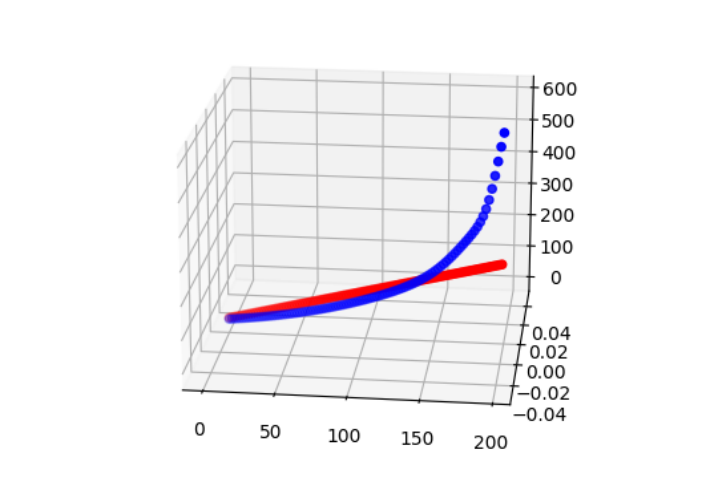
\includegraphics[width=0.4\textwidth]{gambar/hasil_1.png}
  
    % Ubah sesuai dengan keterangan gambar yang diinginkan.
    \caption{Hasil Kalibrasi Kamera Lama.}
    \label{fig:hasilkalibrasilama}
    \begin{enumerate}
      \item \textbf{Warna Merah}: Merupakan koordinat titik pada kamera omnivision. 
      \item \textbf{Warna Biru}: Merupakan koordinat titik pada dunia nyata.
    \end{enumerate}
\end{figure} 

\subsection{Visualisasi Data Kalibrasi Baru}
\label{subsec:visualisasidatakalibrasibaru} 

Hasil dari kalibrasi kamera akan divisualisasikan dalam bentuk grafik 3D. Dalam grafik tersebut, terdapat dua elemen yaitu koordinat titik pada kamera dan koordinat titik pada dunia nyata. 
\begin{figure}[ht]
  \centering
  % Ubah sesuai dengan nama file gambar dan ukuran yang akan digunakan.
  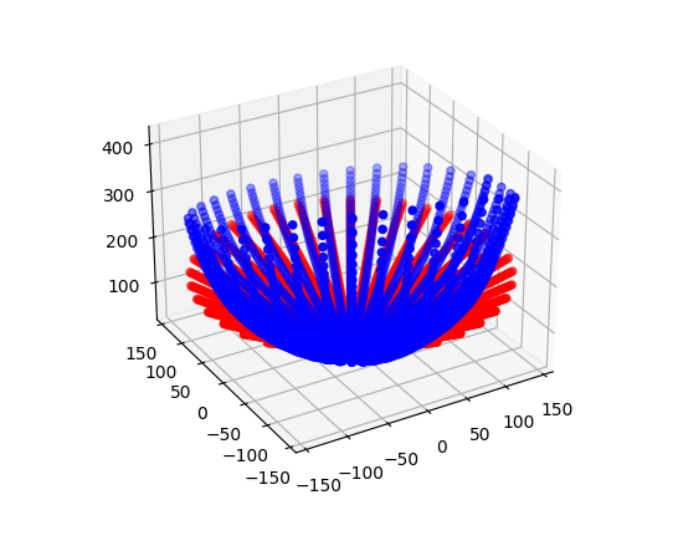
\includegraphics[width=0.4\textwidth]{gambar/hasil_360.png}

  % Ubah sesuai dengan keterangan gambar yang diinginkan.
  \caption{Hasil Kalibrasi Kamera Baru.}
  \label{fig:hasilkalibrasibaru}
  \begin{enumerate}
    \item \textbf{Warna Merah}: Merupakan koordinat titik pada kamera omnivision. 
    \item \textbf{Warna Biru}: Merupakan koordinat titik pada dunia nyata.
  \end{enumerate}
\end{figure} 

\subsection{Pembahasan Perbedaan Hasil Kalibrasi}
\label{subsec:pembahasanperbedaanhasilkalibrasi}

Dari hasil visualisasi yang disajikan dari dua metode Kalibrasi yang berbeda. Dapat dilihat bahwa metode kalibrasi kamera omnivision menggunakan \emph{Machine Learning} lebih baik daripada metode kalibrasi kamera omnivision menggunakan regresi polinomial. Dilihat dari grafik yang dihasilkan, metode kalibrasi kamera omnivision menggunakan \emph{Machine Learning} dapat meng-kalibrasi kamera omnivision pada semua arah. Sedangkan metode kalibrasi kamera omnivision menggunakan regresi polinomial hanya dapat meng-kalibrasi kamera omnivision pada satu arah saja. 


\subsection{Pembahasan Perbedaan Waktu Eksekusi}
\label{subsec:pembahasanperbedaanwaktu}

Selain dari hasil visualisasi yang dihasilkan, perbedaan lainnya adalah waktu eksekusi dari kedua metode kalibrasi. Metode kalibrasi kamera omnivision menggunakan regresi polinomial membutuhkan waktu yang lebih lama daripada metode kalibrasi kamera omnivision menggunakan \emph{Machine Learning}. Hal ini disebabkan karena metode kalibrasi kamera omnivision menggunakan regresi polinomial membutuhkan proses iterasi yang lebih banyak daripada metode kalibrasi kamera omnivision menggunakan \emph{Machine Learning}. 

Berikut adalah perbandingan waktu eksekusi dari kedua metode kalibrasi: 

\begin{figure}
    \centering
    % Ubah sesuai dengan nama file gambar dan ukuran yang akan digunakan.
    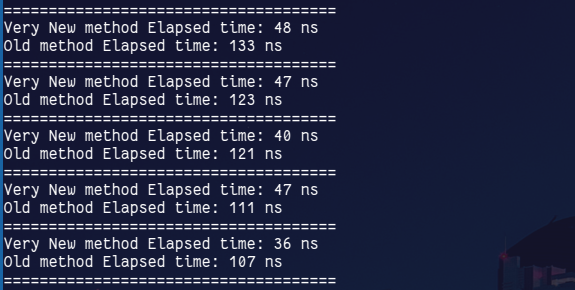
\includegraphics[width=0.4\textwidth]{gambar/beda_waktu.png}
  
    % Ubah sesuai dengan keterangan gambar yang diinginkan.
    \caption{Perbedaan Waktu Eksekusi.}
    \label{fig:bedawaktueksekusi}
\end{figure} 

Waktu eksekusi menggunakan metode regresi polinomial membutuhkan waktu lebih lama dikarenakan pada metode tersebut banyak melakukan proses komputasi perkalian sesuai banyaknya orde polinomial yang digunakan. Sedangkan pada metode \emph{Machine Learning} hanya melakukan akses ke \emph{lookup table} yang sudah dibuat sebelumnya. 

\subsection{Pengujian pada Robot}
\label{subsec:pengujianrobot}

\begin{figure}
    \centering
    % Ubah sesuai dengan nama file gambar dan ukuran yang akan digunakan.
    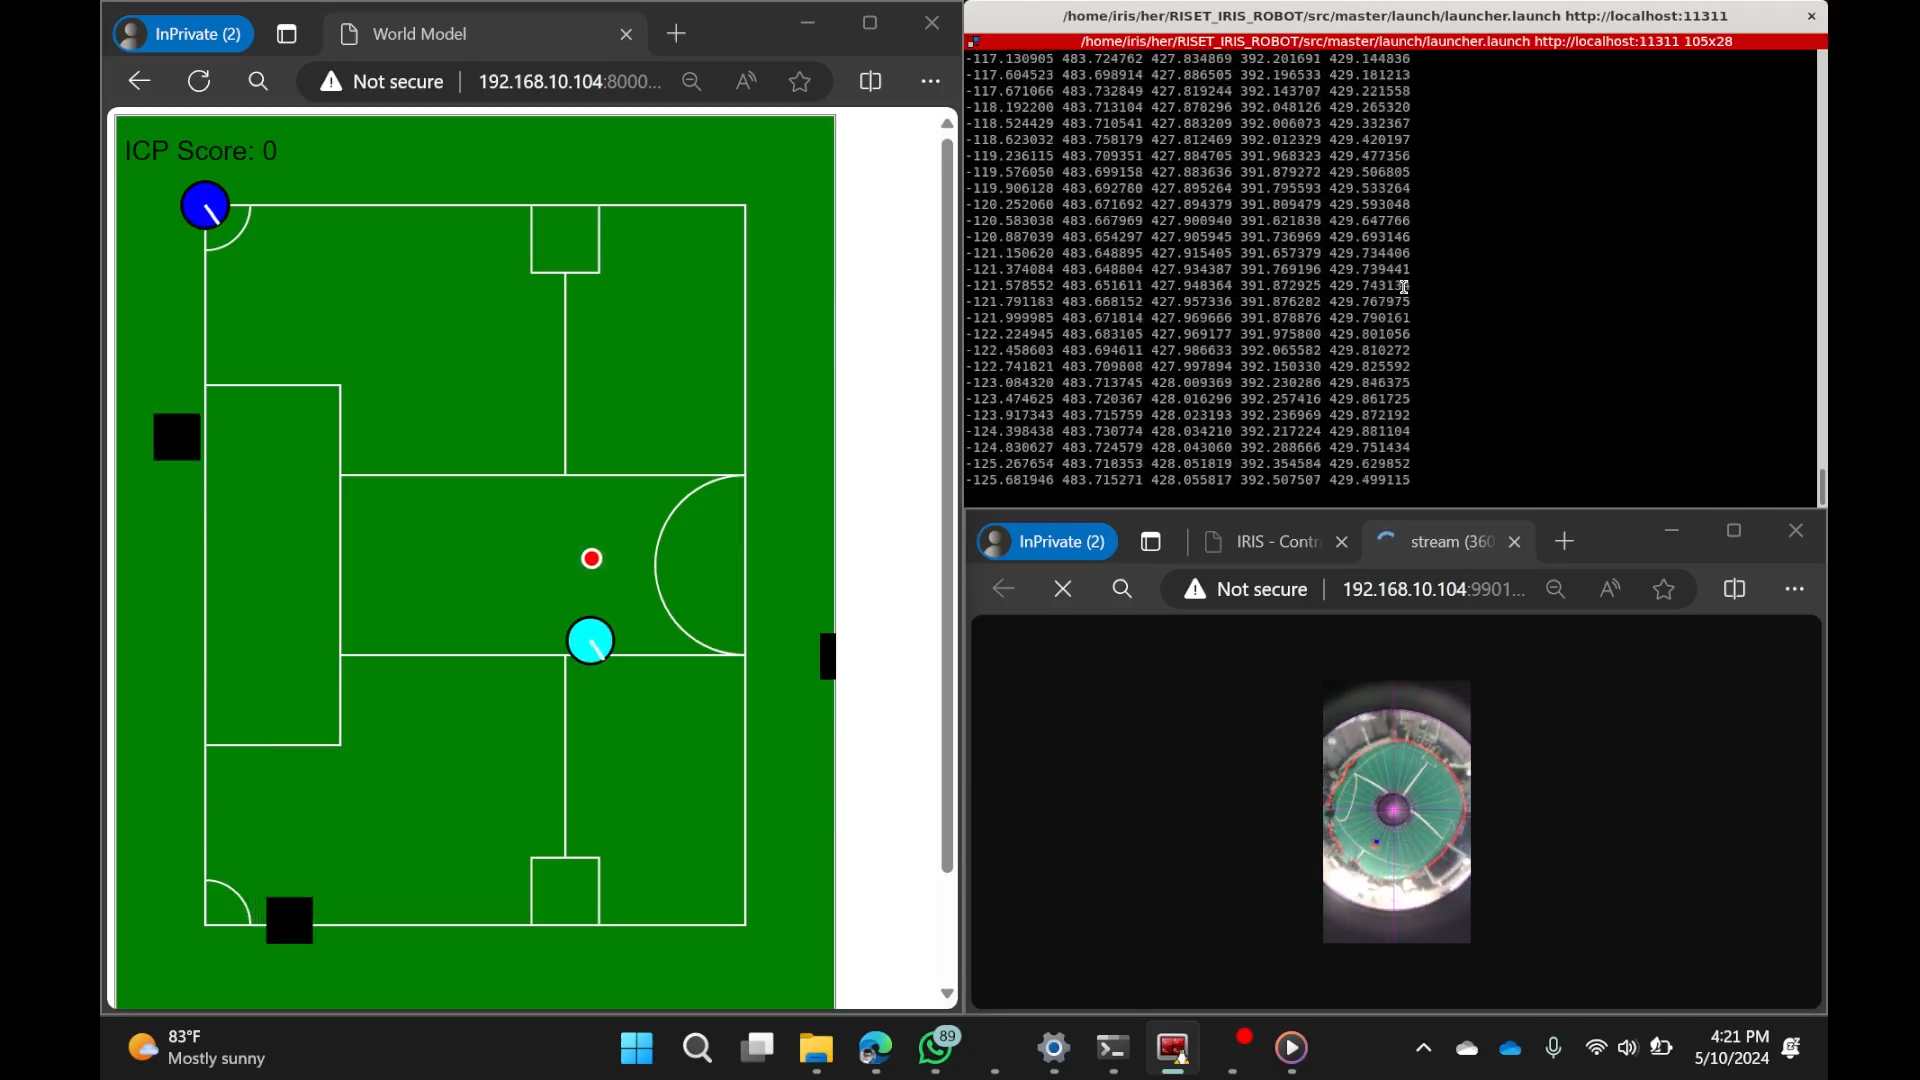
\includegraphics[width=0.4\textwidth]{gambar/saat_putar_bola.png}
  
    % Ubah sesuai dengan keterangan gambar yang diinginkan.
    \caption{Tampilan Robot.}
    \label{fig:tampilanrobot}
\end{figure} 

Pengujian pada robot dilakukan dengan cara mendeteksi bola pada suatu titik lalu memutar robot pada posisinya. Hal itu menyebabkan bola akan terdeteksi melalui berbagi arah yang berbeda. Adapun hasil dari pengujian tersebut adalah sebagai berikut: 

\begin{figure}
    \centering
    % Ubah sesuai dengan nama file gambar dan ukuran yang akan digunakan.
    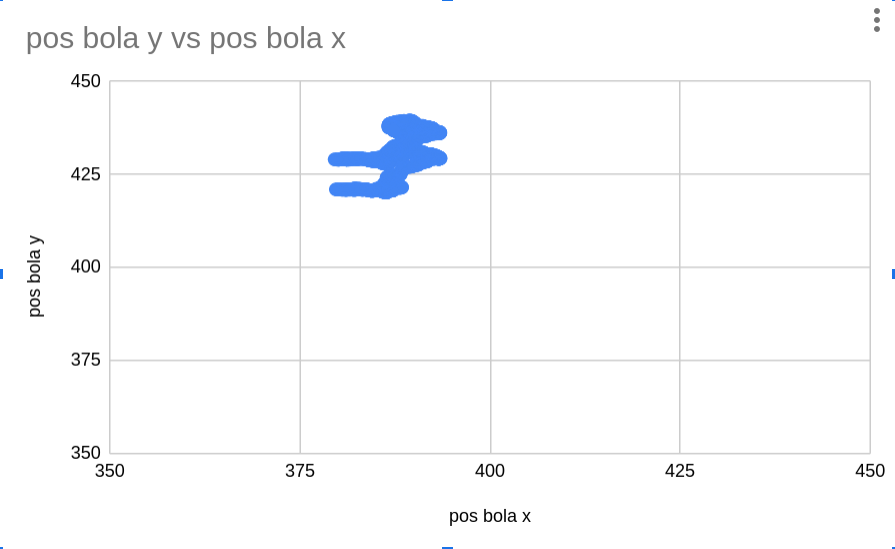
\includegraphics[width=0.4\textwidth]{gambar/putar_bola.png}
  
    % Ubah sesuai dengan keterangan gambar yang diinginkan.
    \caption{Hasil Data Bola.}
    \label{fig:databola}
\end{figure} 

Dapat dilihat bahwa posisi bola relatif sama pada setiap arah yang diberikan.


